% This file was created by matlab2tikz.
%
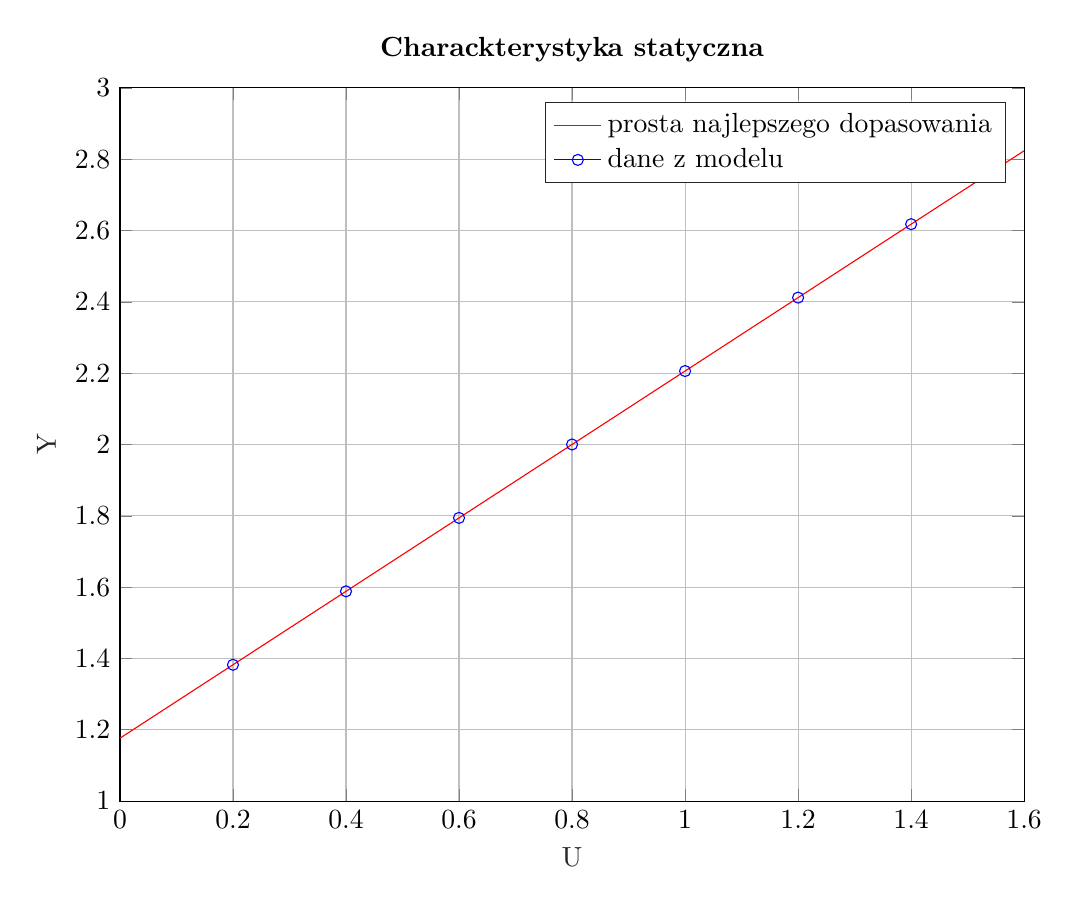
\begin{tikzpicture}

\begin{axis}[%
width=4.521in,
height=3.566in,
at={(0.758in,0.481in)},
scale only axis,
xmin=0,
xmax=1.6,
xlabel style={font=\color{white!15!black}},
xlabel={U},
ymin=1,
ymax=3,
ylabel style={font=\color{white!15!black}},
ylabel={Y},
axis background/.style={fill=white},
title style={font=\bfseries},
title={Charackterystyka statyczna},
xmajorgrids,
ymajorgrids,
legend style={legend cell align=left, align=left, draw=white!15!black}
]
\addplot [color=red]
  table[row sep=crcr]{%
0	1.17631908206646\\
0.1	1.27927919680815\\
0.2	1.38223931154984\\
0.3	1.48519942629154\\
0.4	1.58815954103323\\
0.5	1.69111965577492\\
0.6	1.79407977051661\\
0.7	1.89703988525831\\
0.8	2\\
0.9	2.10296011474169\\
1	2.20592022948338\\
1.1	2.30888034422508\\
1.2	2.41184045896677\\
1.3	2.51480057370846\\
1.4	2.61776068845015\\
1.5	2.72072080319185\\
1.6	2.82368091793354\\
};
\addlegendentry{prosta najlepszego dopasowania}

\addplot [color=blue, draw=none, mark=o, mark options={solid, blue}]
  table[row sep=crcr]{%
0.2	1.38223931154985\\
0.4	1.58815954103323\\
0.6	1.79407977051661\\
0.8	2\\
1	2.20592022948339\\
1.2	2.41184045896677\\
1.4	2.61776068845015\\
};
\addlegendentry{dane z modelu}

\end{axis}
\end{tikzpicture}%